\subsection{Warunki graniczne dla r. Laplace'a}

\begin{frame}{Warunki graniczne dla r. Laplace'a}
  % Sztuczny slajd, jest tu tylko po to, by zaprezentować najpierw tytuł podsekcji, a następnie podpodsekcji – inaczej nikt się nie zorientuje, że zagadnienie Neumanna to też warunek graniczny Laplace'a.
  Rozważymy:
  \begin{itemize}
    \item zagadnienie Dirichleta
    \item zagadnienie Neumanna
    \item zagadnienie Robina
  \end{itemize}
\end{frame}

\subsection*{Warunki graniczne dla r. Laplace'a -- zagadnienie Dirichleta}
\subsubsection{Zagadnienie Dirichleta}

\begin{frame}{Zagadnienie Dirichleta}
  \begin{block}{Zagadnienie Dirichleta}
    mając:
    \begin{itemize}
      \item $G$ -- ograniczony zbiór punktów
      \item $R$ -- wnętrze $G$; $R$ -- jednospójny
      \item $S$ -- brzeg obszaru $R$; $S$ -- odcinkami regularny
      \item $f(x,y)$ -- dana funkcja ciągła na $S$
    \end{itemize}
    należy znaleźć funkcję $u(x,y)$:
    \begin{itemize}
      \item określoną i ciągłą na $R \bigcup S$
      \item identyczną z $f(x,y)$ na $S$
      \item harmoniczną na $R$
    \end{itemize}
  \end{block}
\end{frame}

\begin{frame}
  \begin{columns}
    \column{0.45 \linewidth}
      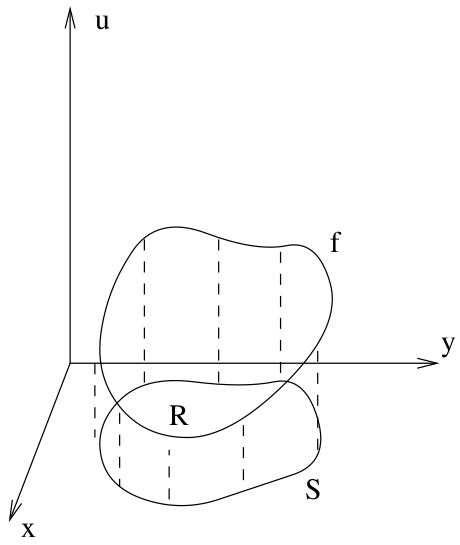
\includegraphics[width = \linewidth]{img/23/dirichlet}
    \column{0.45 \linewidth}
      \begin{itemize}
        \item graf $f(x,y)$ -- w 3D -- zamknięta krzywa
        \item graf $u(x,y)$ -- powierzchnia nad $R \bigcup S$, zawiera $f$
        \item $f$ -- brzeg
      \end{itemize}
  \end{columns}
\end{frame}

\begin{frame}
  Dowodzi się:
  \begin{itemize}
    \item istnienia i jednoznaczności rozwiązania zagadnienia Dirichleta
    \item $S$: prostokąt -- rozwiązanie -- szeregi Fouriera, \\
    okrąg, elipsa -- całka Poissona, szeregi Fouriera \\
    (i gdy można zastosować przekszt. konforemne) \\
    ale: \textit{często rozwiązania analityczne -- wolnozbieżne}
    % Powyższe zdecydowanie powinno być zagnieżdżoną listą wypunktowaną, ale nie rozumiem struktury logicznej – czego dotyczy nawias?
  \end{itemize}

  W większości przypadków -- brak rozwiązań analitycznych (zamkniętych).
\end{frame}

\subsection*{Warunki graniczne dla r. Laplace'a -- zagadnienie Neumanna}
\subsubsection{Zagadnienie Neumanna}

\begin{frame}{Zagadnienie Neumanna}
  \begin{block}{Zagadnienie Neumanna}
    Wyznaczyć $u(x,y)$:
    \begin{itemize}
      \item ciągłą na $R \bigcup S$
      \item harmoniczną na $R$
      \item taką, że jej pochodna w kierunku normalnej wewnętrznej w~każdym punkcie $P$ brzegu $S$ przyjmuje zadane wartości:
      $$\frac{{\partial}u(x,y)}{{\partial}n} = g(x,y)$$
    \end{itemize}
  \end{block}
  Zagadnienie ma jednoznaczne rozwiązanie z dokładnością do stałego składnika.
\end{frame}

\subsection*{Warunki graniczne dla r. Laplace'a -- zagadnienie mieszane; Robina; trzeciego rodzaju}
\subsubsection{Zagadnienie mieszane; Robina; trzeciego rodzaju}

\begin{frame}{Zagadnienie mieszane; Robina; trzeciego rodzaju}
  \begin{block}{Zagadnienie mieszane; Robina; trzeciego rodzaju}
    $$\frac{{\partial}u}{{\partial}n} + H \cdot (u - h) = 0$$
    gdzie $H$,$h$ -- zadane funkcje
  \end{block}
  Powyższe zag. \textit{zag. brzegowe wewnętrzne} % Co za zag. zag.??? Mają być dwa??? (zagwarantuje, zagadnienie)??? A może należy zatytułować ten blok "zagadnienia brzegowe wewnętrzne" zamiast "zag. mieszane (...)"???
\end{frame}

\begin{frame}
  \begin{block}{Zagadnienia brzegowe zewnętrzne}
    Poszukiwana funkcja $u$ powinna być harmoniczną w obszarze nieograniczonym, położonym na zewnątrz powierzchni $S$.
  \end{block}
\end{frame}

\begin{frame}
  Podejście -- transformacja inwersja
  \begin{columns}
    \column{0.45 \linewidth}
      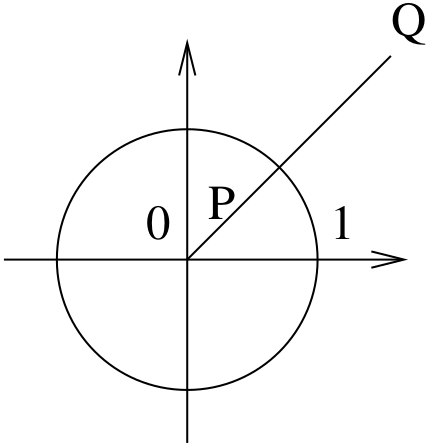
\includegraphics[width = \linewidth]{img/23/inwersja}
    \column{0.45 \linewidth}
      $$|0P| \cdot |0Q| = 1$$
  \end{columns}

  \vspace{5px}

  Zagadnienia brzegowe zewnętrzne mają jednoznaczne rozwiązania; brak ogólnej metody wyznaczania rozwiązań analitycznych.
\end{frame}
